\chapter{The Experiment}

\begin{figure}[h]
\centering
\begin{subfigure}[b]{0.8\textwidth}
                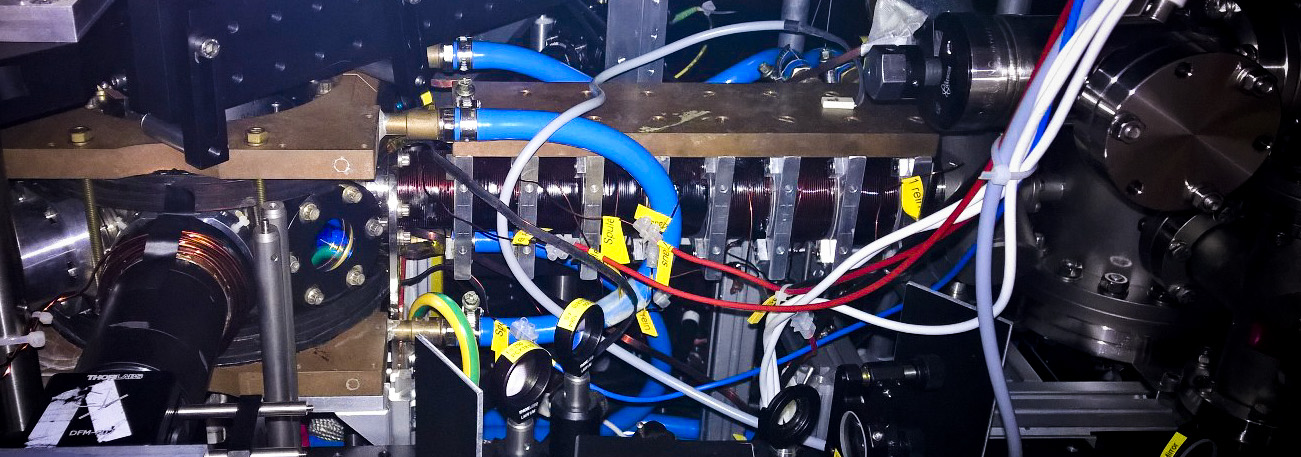
\includegraphics[width=\textwidth]{experiment}
\end{subfigure}
\caption{Photograph of the core-part of the experiment. On the left the octagon-shaped vacuum chamber is visible, with viewports and lenses, focussing beams for the optical dipole trap and the \textsc{mot}. On the right one can see the oven and the Zeeman-slower connecting both parts.}
\label{experiment}
\end{figure}
The experiment in whose framework this thesis is made is using cold Lithium-6 atoms to study few body systems and perform quantum simulation. The approach is to construct fundamental building blocks for systems like superfluids, superconductors and other models in the field of many-body effects. The key feature of the experiment is the possibility to prepare few atoms in a microscopic dipole trap with high control over their number and over their respective interactions using Feshbach resonances.

After vaporizing Lithium in an oven, the first stage of the experiment is the Zeeman slower. When leaving the oven, the atoms are very hot and propagate at relativly high velocities, that are too large to trap them in the \textsc{mot} or dipole trap. The Zeeman-slower reduces this speed using radiation pressure while adapting for the the different doppler shifts, exploiting the Zeeman-effect. The slower is essentially a large tube behind the oven shutter surroundet by coils, that provide a different magnetic field value at every point of the apperatus. A strong laserbeam is pointing along the slower. When the beam is in resonance with an atomic tranition, the photons get absorbed and are pushed in this direction, and  because the spontanious emission is directed in random directions, this leads to slowin of the cloud. The problem now is, that due to the Doppler-effect the atoms see the light blue detuned when flying at high velocities. If the frequency of the laser-beam is adapted to match the resonance frequency for the respective speed, the atoms will be slowed down at first, but will no longer absorb photons because of the now different Doppler shift. Therefore at each point of the Zeeman-slower a magnetic field shifts the atomic levels to match the frequncy of the laser everywhere along the legth of the tube. When leaving the slower the atoms are cold enough to be trapped in the magneto-optical trap. It consists of six counterpropagating near-resonsant laser-beams that, like the Zeeman slower, transfer momentum onto the atoms for a certain velocity. The usage of many retroreflected beams in different directions make it possible to not only force the atoms in a certain direction but to affect all of them with a high absolute speed value and push in the opposite way, in this manner reducing the overall average-speed and therefore cooling the gas. The remaining problem is the drift of cold atoms, because the force of the laserbeams alone is only velocity-dependent and slow particles exit the center of the crossed beams over time. That is why in a magneto-optical trap a magnetic quadrupole-field is applied, that has zero strength in the middle and will increase when moving further away from the center. Therefore the Zeeman-effect shifts the level-distace for the outmoving atoms towards the frequency of the laser, which will then apply a force, dependent on the spatial position, enabeling not only cooling but trapping and compression of the gas-sample. Farther detuning will enable the \textsc{mot} to influence a bigger portion of the atoms, because the point where the magnetic field shifts the transition lines towards the resonance will move outwards. On the other hand will lower detuning increase the density of the cloud, since in that gradient of the radiation pressure will incrase. The limits of temperature for the \textsc{mot} lie in the method of laser-cooling. An absorbed photon always transports the same momentum and sets a minimum for the kinetic energy of the trapped atoms. This limit corresponds to a temperature of around 500 \mu K. The \textsc{mot} used in this experiment can store around 10⁸ atoms. The temperature however has to be reduced much further to match the requirements of the experiment later on. The next step on this ladder is the crossed dipole trap. \begin{figure}[h]
\centering
\begin{subfigure}[b]{0.8\textwidth}
                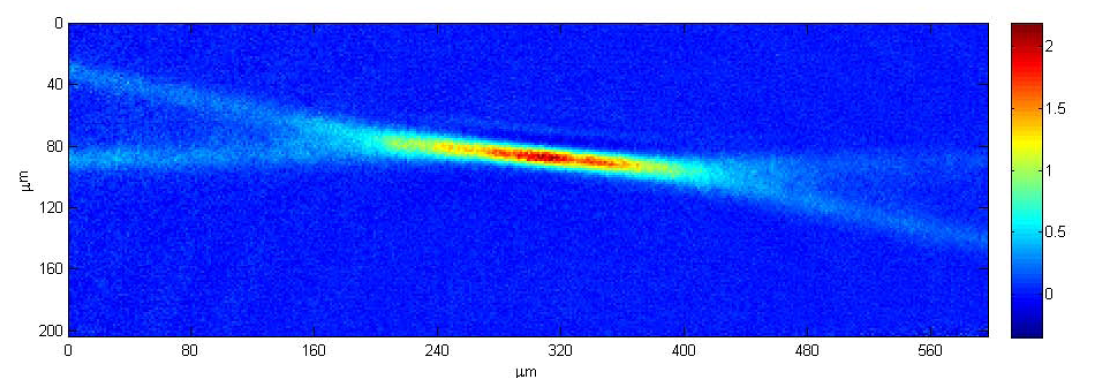
\includegraphics[width=\textwidth]{dipolefoto}
\end{subfigure}
\caption{Absorbtion image of the crossed dipole trap \cite{lompe}.}
\label{experiment}
\end{figure}
It consists of the laserbeam of a 200W Ytterbium fiber-laser (\textsc{ipg ylr-200-lp}) that is far red-detuned from the atomic transitions at 1070 nm. The beams focus lies within the \textsc{mot} to trap as many atoms as possible, with a waist of approximately 40 \mu m (more on that in the meassurement-section). After leaving the vacuum chamber a mirror system guides it back in at an angle. This accounts for the special cross shape of the trap. To trap the most atoms possible the laser is ramped up to full power, leading to a trap depth of over 3 mK. To further cool the sample the power is slowly ramped down. The hottest atoms escape the potential and the rest of the cloud thermalises at a lower temperature. The experiment is then carried out in the so called microtrap, formed by a small, tightly focussed infrared laser-beam at 1064 nm, that intersects the crossed dipole-trap. The small dimensions of the trap result in high spacing between the allowed harmonic vibrational levels. After loading atoms in this microtrap the crossed dipole-trap can be shut down. To control the atom number in the microtrap, a magnetic field gradient distorts the dipole-potential. That leads to the escape of all atoms above a certain level and using this technique one can control the number of atoms between 0 and 10 atoms with high preperation fiddelity. To see the atoms, the microtrap is shut down and the remaining atoms are again trapped in a smaller \textsc{mot}. The resulting flourescence is caught by an objective and projected at the sensor of a \textsc{ccd}-camera. 


